%Inhalt
\section*{Hallo} Jetzt geht's los...

\textbf{fetter Text} \footnote{Text}

Motormanagement Sensoren (\textcite{schneehage:2021:motormanagement}).

Quelle \footnote{\textcite{kofler:2018:hacking}}.

\section{Welche Zeichen dürfen verwendet werden?}

Ziffern: 0…9
Buchstaben: a…z A…Z\\
Sonderzeichen:  . : ; , ? ! ( ) [ ] + - * / = @\\
Steuerzeichen: \$ \& \% \# \_ \{ \} \textasciitilde \textasciicircum \textbackslash \textbar \\
Umlaute: ä ö ü ß Ä Ö Ü\\
Anführungszeichen: "`Hallo!"' ``Hello!'' "<Salut!">\\
Gedankenstrich: - -- \\
EURO-Symbol: \euro

\section{Abstand}

Text

\smallskip etwa $\frac{1}{4}$ Zeile Abstand

\medskip etwa $\frac{1}{2}$ Zeile Abstand

\bigskip etwa $1$ Zeile Abstand

\vspace{2ex} %Relative Maßangabe: für Höhen

Abstand durch vspace

Text \hspace{2em} Abstand durch hspace%Relative Maßangabe:  für Breiten

Abstand durch Leerzeile

\section{Farbe}

\textcolor{red}{Text} \colorbox{red}{\textcolor{white}{Text}}
\textcolor{blau}{Text} \colorbox{blau}{\textcolor{white}{Text}}
\textcolor{orange}{Text} \colorbox{orange}{\textcolor{white}{Text}}
\textcolor{gray}{Text} \colorbox{gray}{\textcolor{white}{Text}}
\textcolor{purple}{Text} \colorbox{purple}{\textcolor{white}{Text}}

\section{Code}

\begin{lstlisting}[language={[LaTeX]TeX}]
% HalloWelt.tex
\documentclass{article}
\begin{document}
	Hallo Welt!
\end{document}
\end{lstlisting}

\begin{lstlisting}[language={C}]
// HalloWelt.c
#include <stdio.h>
int main(void){
	printf("Hallo Welt!\n");
	return 0;
}
\end{lstlisting}

\section*{Mathe}
 
 $x^{2} + px + q = 0$

\begin{equation}
 x_{1,2} = -\frac{p}{2} \pm \sqrt{D}
\end{equation}
 
\begin{align*}
(a+b)^{2}  &= (a+b) (a+b) \\
                &= a^{2} + ab + ba + b^{2} \\
                &= a^{2} + 2ab + b^{2}
\end{align*}

Dezimaltrennzeichen: $1,23$ $1.23$

Exponenten, Indizes, Vektor: $x_{1} \,  x^{2} \, \vec{x}$

\begin{equation}
x = y^{-1} \text{ für alle $y > 0$ }
\end{equation}

Griechische Buchstaben: $\alpha \, \Omega$

Mathematische Symbole: $\le \, \sim \, \ne \, \approx \, \notin$

$\ldots \, \cdots \, \{ \, \} \rightarrow \, \left( \frac{x+a}{x-a} \right)^2$

Brüche, Wurzeln, Binomialkoeffizienten, Summen, Grenzwerte

$\frac{1}{2} \, \frac{x^2}{x^2+1} \, \sqrt{x} \, \sqrt[4]{x^2+1} \, \binom{n}{k} \, \sin x \, \sum\limits_{i=1}^{n} i \, \lim\limits_{x \to 0}$

Matrizen und Fallunterscheidungen

$\boldsymbol{A} = \left(
	\begin{matrix} 
		1 & 2 & 3 \\
		4 & 5 & 6 \\
		7 & 8 & 9
	\end{matrix} 
\right)$

$
f(x) =
\begin{cases}
	   -x  & \text{f"ur $x < 0$} \\
	    1  & \text{f"ur $x = 0$} \\
	\ln x  & \text{f"ur $x > 0$}
\end{cases}
$

$\boxed{E=mc^2}$




\section{Boxen}

\fbox{Text}

\fbox{Text Text \raisebox{-1.0ex}{ Text nach unten } \raisebox{1.0ex}{ Text nach oben } Text Text}

\fbox{
\begin{tabular}{cp{5cm}}
$A \cap B$ &
$A$ und $B$ treten gleichzeitig ein.\\
$A \cup B$ &
Es tritt $A$ oder es tritt $B$ ein
(beide zugleich sind möglich).
\end{tabular}
}

 \section{Bild}
 
 \fbox{

\includegraphics[height=6cm,angle=30]{images/Logo/Logo1.pdf}

\includegraphics[height=4cm,angle=-30]{images/Logo/Logo2.pdf}
 }


Bild (\autoref{fig:bild}).
\begin{figure}[!h]% hier: !hb
	\centering
	
\includegraphics[width=.55\textwidth]{images/Logo/logo.eps}
	\caption{Bild}\label{fig:bild}%% anpassen
\end{figure}
 
 
 \section{Links}
 
 PDF öffnen: (\url{images/Logo/Logo-Details.pdf}) 
 
 Video öffnen: \movie[externalviewer]{(video.mov)}{images/Video/video.mov}
 
 Audio öffnen: \movie[externalviewer]{(H01-Gl-ET.m4a)}{images/Hoertext/H01-Gl-ET.m4a}
 
 Website \footnote{\url{http://bw-ju.de/}}

\section{Tabelle}

% Tab 1
(siehe \autoref{tab:heisetabelle}).
\begin{table}[ht]
\centering
\begin{tabular}{cc}
\toprule 
\textbf{Begriff} & \textbf{Definition}\\
\midrule  
A	&	Text \\
B	&	Text \\ 
C	&	Text \\
D	&	Text \\
E	&	Text \\
F	&	Text \\
\bottomrule
\end{tabular}
\caption{Beschreibung der Tabelle}
\label{tab:heisetabelle}
\end{table}


% Tab 2
\rowcolors{1}{}{grau2}% EIN: oder \showrowcolors o. \hiderowcolors
\begin{table}[h]
\centering
\begin{tabular}{cp{3.5cm}}
\textbf{Begriff} & \textbf{Definition}\\
\hline %\showrowcolors %\hiderowcolors
A	&	Text \\
B	&	Text \\ 
C	&	Text \\
D	&	Text \\
E	&	Text \\
F	&	Mehrzeiliger Text \newline in einer Zelle \\
\end{tabular}
\caption{Beschreibung}
\label{tab:tabelle}
\end{table}
\rowcolors{1}{}{}% AUS

%\newpage
%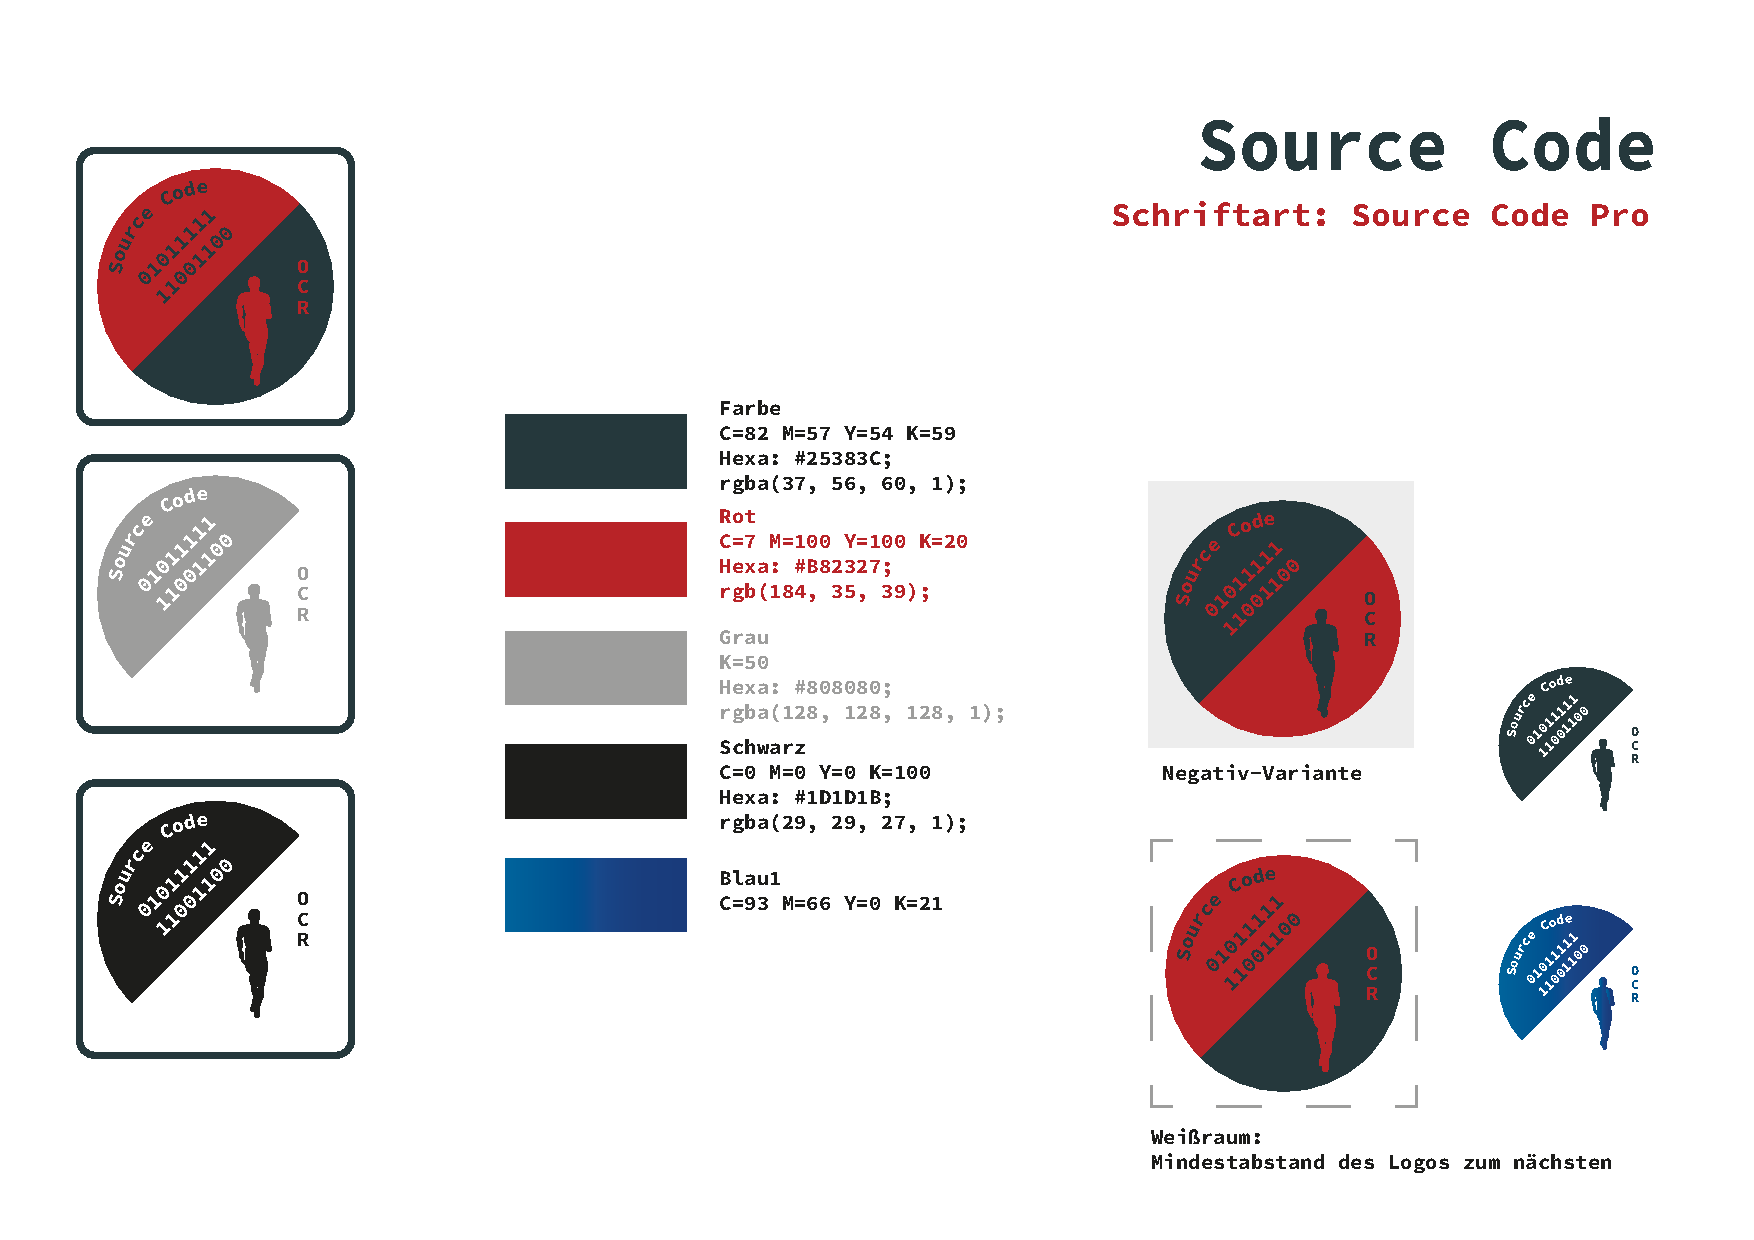
\includepdf[pages=-,landscape]{images/Logo/Logo-Details.pdf}%landscape
